\documentclass{scrreprt}

\usepackage{aligned-overset}
\usepackage{amsmath}
\usepackage{amsthm}
\usepackage{amssymb}
\usepackage{bm}
\usepackage[inline,shortlabels]{enumitem}
\usepackage{hyperref}
\usepackage[utf8]{inputenc}
\usepackage{multicol}
\usepackage{mathtools}
\usepackage{pdflscape}
\usepackage{physics}
\usepackage{tabularx}
\usepackage[table]{xcolor}
\usepackage{titling}
\usepackage{fancyhdr}
\usepackage{xfrac}
\usepackage{pgfplots}

\pgfplotsset{compat = newest}
\usepgfplotslibrary{fillbetween}
\usetikzlibrary{calc}


\author{Karsten Lehmann}
\date{SoSe 2025}
\title{Übungsblatt 04\\INF-B-120, Mathematische Methoden für Informatiker}

\setlength{\parindent}{0pt}

\setlength{\headheight}{26pt}
\pagestyle{fancy}
\fancyhf{}
\lhead{\thetitle}
\rhead{\theauthor}
\lfoot{\thedate}
\rfoot{Seite \thepage}

\begin{document}
\paragraph{Ü 4.1} Es werden die folgenden Funktionen
$f \colon D\qty\big(f) \to \mathbb{R}$ betrachtet:

\begin{enumerate*}[(a)]
\item $f\qty\big(x) = \frac{\sqrt{1 - x^2}}{x}$
\item $f\qty\big(x) = \ln\qty(1 + \frac{1}{x - 1})$
\item $f\qty\big(x) = \frac{x^2 - x - 6}{x + 2}$
\end{enumerate*}

Dabei bezeichnet $D\qty\big(f) \subseteq \mathbb{R}$ die größte Menge, auf der
$f$ definiert werden kann.

\begin{itemize}
\item Bestimmen Sie $D\qty\big(f)$ für jede der Funktionen.
\item Finden Sie alle Unstetigkeitsstellen der Funktionen, falls solche existieren
\item Sind die Funktionen injektiv?
  Sind sie surjektiv?
  Begründen Sie ihre Antworten!
\end{itemize}

\subparagraph{Lsg.}

\begin{enumerate}[(a)]
\item \phantom{\null} \\
  \begin{tikzpicture}[scale=1]
    \begin{axis}[
      axis x line=center,
      axis y line=center,
      grid=both,
      samples=200,
      xmin=-1.5,
      xmax=1.5,
      xtick distance=1,
      ymin=-10.5,
      ymax=10.5,
      ytick distance=5,
    ]
      \addplot[domain=-1:-0.01, smooth] { (sqrt(1 - \x * \x) / \x) };
      \addplot[domain=0.01:1, smooth] { (sqrt(1 - \x * \x) / \x) };
    \end{axis}
  \end{tikzpicture}

  Es ist $D\qty\big(f) = \qty\big[-1, 1] \setminus \qty\big{0}$, da der
  Nenner des Bruchs nicht negativ sein kann und die Wurzel nur für Werte größer
  oder gleich Null definiert ist.

  Nun ist die Funktion stetig auf $D\qty\big(f)$, das sie eine Komposition
  stetiger Funktionen ist.
  ($x = 0$ liegt nicht in $D\qty\big(f)$).

  Außerdem ist die Funktion nicht injektiv, da
  $f\qty\big(-1) = 0 = f\qty\big(1)$.

  Sei nun $y \in \mathbb{R}$ beliebig.
  Dann ist
  \begin{flalign*}
    y = \frac{\sqrt{1 - x^2}}{x} &\iff yx \overset{x \ne 0}{=} \sqrt{1 - x^2} \\
                                 &\iff y^2x^2 = 1 - x^2 \\
                                 &\iff y^2 = \frac{1}{x^2} - 1 \\
                                 &\iff y^2 + 1= \frac{1}{x^2} \\
                                 &\iff \pm\sqrt{y^2 + 1} = \frac{1}{x} \\
                                 &\iff x = \pm \frac{1}{\sqrt{y^2 + 1}} \\
  \end{flalign*}
  \textbf{Probe:} Es ist
  \begin{flalign*}
    f\qty(\frac{1}{\sqrt{y^2 + 1}})
    &= \frac{\sqrt{1 - \qty(\frac{1}{\sqrt{y^2 + 1}})^2}}{\frac{1}{\sqrt{y^2 + 1}}} \\
    &= \frac{\sqrt{1 - \frac{1}{y^2 + 1}}}{\frac{1}{\sqrt{y^2 + 1}}} \\
    &= \sqrt{1 - \frac{1}{y^2 + 1}} \cdot \sqrt{y^2 + 1} \\
    &= \sqrt{\frac{y^2 + 1}{y^2 + 1} - \frac{1}{y^2 + 1}} \cdot \sqrt{y^2 + 1} \\
    &= \sqrt{\frac{y^2}{y^2 + 1}} \cdot \sqrt{y^2 + 1} \\
    &= \frac{y}{\sqrt{y^2 + 1}} \cdot \sqrt{y^2 + 1} \\
    &= \abs{y}
  \end{flalign*}
  und
  \begin{flalign*}
    f\qty(-\frac{1}{\sqrt{y^2 + 1}})
    &= -\frac{\sqrt{1 - \qty(-\frac{1}{\sqrt{y^2 + 1}})^2}}{\frac{1}{\sqrt{y^2 + 1}}} \\
    &= -\frac{\sqrt{1 - \frac{1}{y^2 + 1}}}{\frac{1}{\sqrt{y^2 + 1}}} \\
    &= -\sqrt{1 - \frac{1}{y^2 + 1}} \cdot \sqrt{y^2 + 1} \\
    &= -\sqrt{\frac{y^2 + 1}{y^2 + 1} - \frac{1}{y^2 + 1}} \cdot \sqrt{y^2 + 1} \\
    &= -\sqrt{\frac{y^2}{y^2 + 1}} \cdot \sqrt{y^2 + 1} \\
    &= -\frac{y}{\sqrt{y^2 + 1}} \cdot \sqrt{y^2 + 1} \\
    &= -\abs{y}
  \end{flalign*}
  Somit ist $f\qty\big(x)$ mit $\begin{cases}
    \frac{1}{\sqrt{y^2 + 1}} & y > 0 \\
    -\frac{1}{\sqrt{y^2 + 1}} & y \leq 0 \\
  \end{cases}$ surjektiv.

\newpage
\item \phantom{\null} \\
  \begin{tikzpicture}[scale=1]
    \begin{axis}[
      axis equal image,
      axis x line=center,
      axis y line=center,
      grid=both,
      samples=200,
      xmin=-5.5,
      xmax=5.5,
      xtick distance=1,
      ymin=-4,
      ymax=4,
      ytick distance=1,
    ]
      \addplot[domain=-5:1, smooth] { ln(1 + (1 / (\x - 2)))) };
      \addplot[domain=2:5, smooth] { ln(1 + (1 / (\x - 2)))) };
    \end{axis}
  \end{tikzpicture}

  Der Logarithmus ist nur für Funktionswerte größer als Null definiert.
  Es folgt
  \[
    1 + \frac{1}{x - 2} > 0 \iff \frac{1}{x - 2} > -1
  \]

  \begin{minipage}{.45\textwidth}
    \textbf{Falls} $x - 2 < 0$, also $x < 2$

    \begin{flalign*}
      1 < -1 \cdot \qty\big(x - 2) &\iff 1 < 2 - x \\
                                   &\iff -1 < -x \\
                                   &\iff 1 > x
    \end{flalign*}
  \end{minipage}
  \begin{minipage}{.45\textwidth}
    \textbf{Falls} $x - 2 \geq 0$, also $x \geq 2$

    \begin{flalign*}
      1 > -1 \cdot \qty\big(x - 2) &\iff 1 > 2 - x \\
                                   &\iff -1 > -x \\
                                   &\iff 1 < x
    \end{flalign*}
  \end{minipage}

  $\Rightarrow D\qty\big(f) = \qty\big(-\infty, 1) \cap \qty\big(2, \infty)$

  Nun ist die Funktion $f$ als Komposition stetiger Funktionen auf $D\qty\big(f)$
  ebenfalls stetig.

  Weiter sind sowohl $\ln\qty\big(x)$ als auch $1 + \frac{1}{x - 2}$ injektiv.
  Somit ist $f$ injektiv.
  Allerdings ist $f$ nicht surjektiv, da der Logarithmus eine Bijektion ist,
  allerdings $1 - \frac{1}{x - 2} \ne 1$ für alle $x \in \mathbb{R}$.
  Damit hat $\ln\qty\big(1)$ kein Urbild.
\end{enumerate}

\newpage
\paragraph{Ü 4.2}
\begin{enumerate}[(a)]
\item Untersuchen Sie, ob die gegebenen reellen Funktionen an der Stelle $x = 2$
  stetig sind.
  \begin{enumerate}[(1)]
  \item $f\qty\big(x) = \begin{cases}
      e^{x - 2} & \text{für } x < 2 \\
      2 - \frac{1}{x} & \text{für } x \geq 2 \\
    \end{cases}$.

    \subparagraph{Lsg.}\phantom{\null} \\
    \begin{tikzpicture}[scale=1]
      \begin{axis}[
        axis equal image,
        axis x line=center,
        axis y line=center,
        grid=both,
        samples=200,
        xmin=-0.5,
        xmax=5.5,
        xtick distance=1,
        ymin=-0.5,
        ymax=5.5,
        ytick distance=1,
      ]
        \addplot[domain=0:2, smooth] { e^(2 - x) };
        \addplot[domain=2:5, smooth] { 2 - (1 / \x) };

        \node[circle, draw, fill, minimum size=2pt, inner sep = 0pt] at (2, 1.5) {};
      \end{axis}
    \end{tikzpicture}

    Es ist $\displaystyle \lim_{x \to 2-} e^{x - 2} = 1$ und
    $\displaystyle \lim_{x \to 2+}2 - \frac{1}{x} = \frac{3}{2}$.
    Damit existiert $\displaystyle \lim_{x \to 2} f\qty\big(x)$ nicht und die
    Funktion hat an $x = 2$ eine Sprung.
  \end{enumerate}

\item Wie müssen die reellen Konstanten $a$ und $b$ gewählt werden, damit die
  stückweise gegebene Funktion $f \colon \mathbb{R} \to \mathbb{R}$ mit
  \[
    f\qty\big(x) = \begin{cases}
      2\qty\big(x + \pi) & x \leq -\frac{\pi}{2} \\
      a \sin x + b & \abs{x} < \frac{\pi}{2} \\
      \qty(x - \frac{\pi}{2})^2 & x \geq \frac{\pi}{2}
    \end{cases}
  \]
  auf ganz $\mathbb{R}$ stetig ist?

  \subparagraph{Lsg.} Seien zuerst $a = 1$ und $b = 0$.
  Dann ist der Graph

  \begin{tikzpicture}[scale=1.1]
    \begin{axis}[
      axis equal image,
      axis x line=center,
      axis y line=center,
      grid=both,
      samples=200,
      xmin=-5.5,
      xmax=5.5,
      xtick distance=1,
      ymin=-3.3,
      ymax=3.5,
      ytick distance=1,
    ]
      \addplot[domain=-5:-1.571, smooth] { 2(x + pi) };
      \addplot[domain=-1.57:1.57, smooth] { sin(deg(x)) };
      \addplot[domain=1.57:5, smooth] { (x - pi/2)^2 };
    \end{axis}
  \end{tikzpicture}

  Nun ist
  $\displaystyle \lim_{x \to -\frac{\pi}{2}-} 2\qty\big(x + \pi) = f\qty(-\frac{\pi}{2}) = \pi$
  und
  $\displaystyle \lim_{x \to \frac{\pi}{2}+} \qty(x - \frac{\pi}{2})^2 = f\qty(\frac{\pi}{2}) = 0$.
  Somit werden $a$ und $b$ gesucht mit
  $\displaystyle \lim_{x \to -\frac{\pi}{2}+} a \sin x + b = \pi$
  und
  $\displaystyle \lim_{x \to \frac{\pi}{2}-} a \sin x + b = 0$.

  Schließlich sind
  \[
    a \sin\qty(-\frac{\pi}{2}) + b = -a + b \iff \pi = b - a
  \]
  und
  \[
    a \sin\qty(\frac{\pi}{2}) + b = a + b \iff 0 = a + b
  \]
  $\Rightarrow a = -\frac{\pi}{2}$ und $b = \frac{\pi}{2}$.
\end{enumerate}

\paragraph{Ü 4.3}
\begin{enumerate}[(a)]
\item Zeigen Sie, dass die rekursive definierte Zahlenfolge
  $\qty(x_n)_{n \in \mathbb{N}}$ mit
  \[
    x_{n + 1} \coloneqq \sqrt{2 + x_n}, \quad x_0 \coloneqq \sqrt{3}
  \]
  für alle $n \in \mathbb{N}$ durch $\sqrt{2} < x_n < 2$ beschränkt ist und
  streng monoton wächst.
  Nutzen Sie dazu die Methode der vollständigen Induktion.
  Begründen Sie, dass die Folge konvergiert und berechnen Sie den Grenzwert
  $\displaystyle a \coloneqq \lim_{n \to \infty} x_n$.

  \subparagraph{Lsg.} Seien
  \[
    P\qty\big(n) \colon \sqrt{2} < x_n < 2
  \]
  und
  \[
    Q\qty\big(n) \colon x_n < x_{n + 1}
  \]
  Nun ist die Behauptung, dass $P\qty\big(n)$ und $Q\qty\big(n)$ für alle
  $n \in \mathbb{N}$ gelten.

  \textbf{Induktionsanfang:}
  $P\qty\big(1) \colon \sqrt{2} < \sqrt{2 + \sqrt{3}} < 2$ und
  Auch $Q\qty\big(1) \colon \sqrt{2 + \sqrt{3}} < \sqrt{2 + \sqrt{2 + \sqrt{3}}}$
  sind offensichtlich wahr.

  \textbf{Induktionsschritt:} Angenommen $P\qty\big(n)$ und $Q\qty\big(n)$ wären
  für ein beliebiges $n \in \mathbb{N}$ wahr (Induktionsvoraussetzung), dann
  gilt für $P\qty\big(n + 1)$
  \[
    P\qty\big(n + 1) \colon \sqrt{2}
    < \sqrt{2 + \sqrt{2}}
    \overset{\text{IV}}
    < \sqrt{2 + x_n} = x_{n + 1}
    \overset{\text{IV}}{<} \sqrt{2 + 2} = \sqrt{4} = 2
  \]
  und für $Q\qty\big(n)$ gilt nach der Induktionsvoraussetzung, dass
  \[
    x_n < x_{n + 1} \iff 2 + x_n < 2 + x_{n + 1} \iff \sqrt{2 + x_n} < 2 + x_{n + 1}
  \]
  Somit impliziert $Q\qty\big(n) \Rightarrow Q\qty\big(n + 1)$.

  Damit folgt die Behauptung aus dem Satz über die vollständige Induktion und
  die Folge konvergiert nach dem Monotoniekriterium.

  \newpage
  Es ist
  \begin{flalign*}
    \lim_{n \to \infty} x_{n + 1}
    &= \lim_{n \to \infty} \sqrt{2 + x_n} \\
    &= \lim_{n \to \infty} \sqrt{\lim_{n \to \infty} 2 + \lim_{n \to \infty} x_n} \\
    &= \sqrt{2 + a}
  \end{flalign*}
  Da nun $\displaystyle a = \lim_{n \to \infty} x_n = \lim_{n \to \infty} x_{n + 1}$
  folgt
  \begin{flalign*}
    a = \sqrt{2 + a}
    &\Rightarrow a^2 = 2 + a \\
    &\Rightarrow 0 = a^2 - a - 2 = \qty\big(a + 1)\qty\big(a - 2) \\
    &\Rightarrow a_1 = 2 \text{ und } a_2 = -1
  \end{flalign*}
  und durch eine Probe fällt schnell auf, dass $a_2$ eine falsche Lösung ist
  und $a = 2$.
\end{enumerate}
\end{document}
